\documentclass[10pt,a4paper]{article}
\usepackage[utf8]{inputenc}
\usepackage[german]{babel}
\usepackage[T1]{fontenc}
\usepackage{amsmath}
\usepackage{amsfonts}
\usepackage{hyperref}
\usepackage{amssymb}
\usepackage{pdfpages}
\usepackage[left=2cm,right=2cm,top=2cm,bottom=2cm]{geometry}

\author{Jonas Betzendahl und Stefan Dresselhaus}
\title{\textbf{Projektausarbeitung der Vorlesung\\Fortgeschrittene Funktionale Programmierung in Haskell}}

\setcounter{secnumdepth}{3}
\parindent0pt

\begin{document}
\maketitle
\tableofcontents
\bigskip\bigskip\bigskip

Im Sommersemester 2015 haben wir, Stefan Dresselhaus und Jonas Betzendahl, an der Universität Bielefeld eine Vorlesung mit dem Namen \glqq Fortgeschrittene Funktionale Programmierung in Haskell\grqq\ gehalten, unter der Aufsicht und mit der Beratung von Dr. Alexander Sczyrba.

Alle Materialien (online verfügbar unter \,\url{https://github.com/FFPiHaskell}) wurden von uns eigenständig erarbeitet, vorbereitet und erstellt. Insgesamt wurden 11 Vorlesungen gehalten, auf die Themen werden wir unten im einzelnen noch genauer eingehen.
\bigskip

Zu jeder Vorlesung, die im Hörsaal gehalten wurde, gibt es ein äquivalentes Video auf YouTube.
Diese sind oftmals direkte Mitschnitte der Vorlesung, in manchen Fällen (z.B. bei technischen Schwierigkeiten) allerdings auch nachträglich erstellte Aufnahmen, die allerdings bis auf wenige und geringe Änderungen die gleichen Inhalte besprechen.

Alle diese Videos sind zu finden unter dem Kanal \glqq Fortgeschrittene Funktionale Programmierung in Haskell\grqq : \;\url{https://www.youtube.com/channel/UC5yZfQZrZnug0sgvveTTfnw}
\bigskip

Alle verwendeten Foliensätze sind im Appendix dieses Dokumentes zu finden und außerdem online verfügbar: \;\url{https://github.com/FFPiHaskell/slides}

\newpage

\section{Einführung}

Als Voraussetzung für die Teilnahme an der Vorlesungen haben wir uns an der Vorlesung \glqq Programmieren in Haskell\grqq\ orientiert, die alle Studierenden der Studiengänge KOI, NWI und BIG sowie alle Studierenden des Nebenfaches in ihrem ersten Semester hören. Allerdings liegt diese Vorlesung bei vielen auch schon eine lange Zeit zurück.

In dieser ersten Vorlesung haben wir deshalb zunächst die Grundlagen von Haskell wiederholt (Syntax, Higher-order-functions, laziness, \dots) und einige Vorgehensweisen erläutert, die beim Programmieren in Haskell nützlich sind (i.e. \glqq thinking in types\grqq\ und \glqq problem solving by composition\grqq).

\smallskip\smallskip
Folien im \hyperref[v1]{Appendix}, Video auf YouTube: \;\url{https://www.youtube.com/watch?v=lDqrgkDJVXo}

\section{Typklassen}

Viele Konzepte der nächsten Vorlesungen und in der Haskell-Programmierung allgemein basieren auf dem Verständnis und der korrekten Instanziierung von verschiedenen Typklassen (so ist zum Beispiel bekannterweise die \texttt{IO}-Monade die einzige Möglichkeit, Seiteneffekte mit einem Haskell-Programm zu erreichen).

In dieser Vorlesung haben wir deshalb einen näheren Blick auf Typklassen in Haskell allgemein und insbesondere auf die Typklassen \texttt{Functor}, \texttt{Applicative} und \texttt{Monad} und auf die dazugehörigen Funktionen geworfen.

\smallskip\smallskip
Folien im \hyperref[v2]{Appendix}, Video auf YouTube: \;\url{https://www.youtube.com/watch?v=EuwgsFJEMMo}

\section{Monad transformers}

Nachdem in der letzten Vorlesung u.a. Monaden näher behandelt wurden, haben wir in dieser Vorlesung den Fokus auf Monadentransformer gelegt. Diese stellen ein Werkzeug dar, dass das Arbeiten in mehreren Monaden zur gleichen Zeit deutlich vereinfacht.

Insbesondere wurde auch der \texttt{RWST} vorgestellt, den Read-Write-State-Transformer, der die Basis für viele Echtweltanwendungen, die in Haskell geschrieben werden, darstellt.

\smallskip\smallskip
Folien im \hyperref[v3]{Appendix}, Video auf YouTube: \;\url{https://www.youtube.com/watch?v=ICmpnVJgRww}

\section{Wiederholung \& Parsing}

Auf Wunsch von einigen Studierenden haben wir einen Teil dieser Vorlesung darafu verwendet, die in den letzten beiden Vorlesungen vorgesetellten Konzepte wie Funktoren, Appliaktive, Monaden und Monadentransformatoren nochmal genauer zu beleuchten.

Parsing ist in der Softwareentwicklung ein wichtiges Feld. In Haskell ist es jedoch mit Bibliotheken wie \texttt{Parsec} oder \texttt{Attoparsec} durch die Verwendung von Parser-Kombinatoren besonders einfach und elegant zu lösen, wie wir im zweiten Teil gezeigt haben. 

\smallskip\smallskip
Folien im \hyperref[v4]{Appendix}, Video auf YouTube: \;\url{https://www.youtube.com/watch?v=k61BzWjzY0s}

\section{Parallelism}

Die Verwendung von mehreren Kernen / Multithreading ist eine der großen Stärken von Haskell, insbesondere, weil es oft leicht fällt den sequentiellen Code zur Lösung eines Problems von dem Code, der den Parallelismus managed, klar zu trennen.

Inhalt dieser Vorlesung waren deshalb verschiedene Herangehensweisen, die Haskell bereit stellt so wie parralel evaluation strategies und die Par-Monade. Außerdem konnten wir kurz auf regular parallel arrays (RePa) und effiziente GPU-Programmierung in Haskell eingehen.

\smallskip\smallskip
Folien im \hyperref[v5]{Appendix}, Video auf YouTube: \;\url{https://www.youtube.com/watch?v=2AEy5Zs0tas}

\section{Concurrency}

Als Fortsetzung zur letzten Vorlesung haben wir den Fokus in dieser Vorlesung auf Concurrency statt auf Parallelism gelegt. Wir haben grundlegendes Threadmanagement besprochen, mehrere Herangehensweisen an Kommunikation zwischen Threads dargelegt (z.B. \texttt{MVars}) und software transactional memory als ein neues Paradigma, dass (trotz hoher Versprechen un) in anderen Sprachen noch nicht oft benutzt wird, vorgestellt.
\smallskip\smallskip

Zur Verfestigung des Gelernten haben wir große Teile der Implementation eines einfachen Chat-Servers gezeigt und beleuchtet, wie die vorher erklärten Konzepte dabei zur Anwendung kommen.

\smallskip\smallskip
Folien im \hyperref[v6]{Appendix}, Video auf YouTube: \;\url{https://www.youtube.com/watch?v=qEsKZBa7ju8}

\section{Lenses \& QuickCheck}

Lenses sind als funktionales Gegenstück zu Gettern und Settern aus OOP ein wichtiger Bestandteil vieler größerer Projekte in Haskell und Bekanntheit mit Lenses wird vielerorts vorausgesetzt. Wir haben deshalb die Funktionsweise und Teile der Implementierung einer simpleren Version hier vorgestellt und hergeleitet.
\smallskip\smallskip

Als zweiten Teil der Vorlesung haben wir das Konzept von property-based testing vorgestellt und die Differenzen sowie Vor- und Nachteile im Vergleich zu klassischen Unit-tests diskutiert.

\bigskip
Folien im \hyperref[v7]{Appendix}, Video auf YouTube: \;\url{https://www.youtube.com/watch?v=N4P0unXq1lo}

\section{Yesod}

Yesod ist eine weithin bekannte Bibliothek für Webdevelopment in Haskell und darüber hinaus Basis für eines der drei Projekte zur Prüfungsleistung des Moduls. Deshalb haben wir in dieser Vorlesung sowhl Grundlagen (Ruten, Quasiquoter) als auch einige fortgeschrittene Konzepte (Implementierung einer eigenen Schnittstelle zur Authentifizierung) der Entwicklung mit Yesod vorgestellt (inkl. live-coding) und gezeigt.

\bigskip
Folien im \hyperref[v8]{Appendix}, Video auf YouTube: \;\url{https://www.youtube.com/watch?v=kLHX6DVVJTA}

\section{Datenstrukturen 1: succinct and cache-oblivious}

Die Haskell-Bibliothek \texttt{Data.Map} stellt seit Jahren bereits einen Bezugspunkt dar, was Performance in Haskell angeht. Allerdings basiert sie intern auf dem RAM-Modell, geht also davon aus, dass alle Zugriffe auf den RAM gleich viel Zeit benötigen, was nicht den Realitäten mit heutiger Hardware entspricht.
\smallskip\smallskip

Der Haskell-Programmierer Edward Kmett hat eine alternative Bibliothek aufgestellt, die Nutzen von succinct und cache-oblivious Datenstrukturen macht. Wir haben in dieser Vorlesung die notwendigen Begriffe eingeführt, die Problematik vorgestellt und uns Teile der Implementierung hergeleitet.

\bigskip
Folien im \hyperref[v9]{Appendix}, Video auf YouTube: \;\url{https://www.youtube.com/watch?v=Bl3bCrrvKBo}

\section{Datenstrukturen 2: finger trees \& laziness}

Als Fortsetzung des Themas \glqq funktionale Datenstrukturen\grqq\ haben wir in dieser Vorlesung einen genaueren Blick drauf geworfen, warum altbekannte Datenstrukturen wie zum Beispiel die doppelt verkettete Liste in Haskell Probleme aufwerfen und Finger Trees als eine effiziente und nützliche Alternative präsentiert.
\smallskip\smallskip

Im zweiten Teil haben wir uns tiefergehend mit dem Konzept der nicht-strikten Evaluierungsstrategie in Haskell (auch bekannt als \glqq laziness\grqq\ oder \glqq lazy evaluation\grqq) auseinander gesetzt und Vor- und Nachteile diskutiert. Diese Strategie bietet ein Alleinstellungsmerkmal der Sprache Haskell und verdient deshalb besondere Beachtung.

\bigskip
Folien im \hyperref[v10]{Appendix}, Video auf YouTube: \;\url{https://www.youtube.com/watch?v=Rj9huPBgc7s}

\section{Lambdakalkül \& Kategorientheorie}

Aufgrund der großen Relevanz (in der Theorie von Programmiersprachen und Berechnung allgemein) seit seinem Entwurf haben wir in dieser Vorlesung das Lambdakalkül behandelt, zunächst beispielhaft behandelt an einem Spiel von Brent Victor.
\smallskip\smallskip

Außerdem wollten wir gerne erreichen, dass die interessierten unter unseren Zuhörern eine
genauere Erläuterung eines sehr beliebten Satzes innerhalb der Haskell-Community (\glqq Monaden sind nur monoide in der Kategorie der Endofunktoren\grqq) bekommen. Deshalb setzt sich der zweite Teil der Vorlesung damit und mit den Voraussetzungen dafür auseinander.

\bigskip
Folien im \hyperref[v11]{Appendix}, Video auf YouTube: \;\url{https://www.youtube.com/watch?v=0bouTdYfrqQ}

\newpage
\section{Appendix}

\subsection*{Vorlesung 1:}
\label{v1}
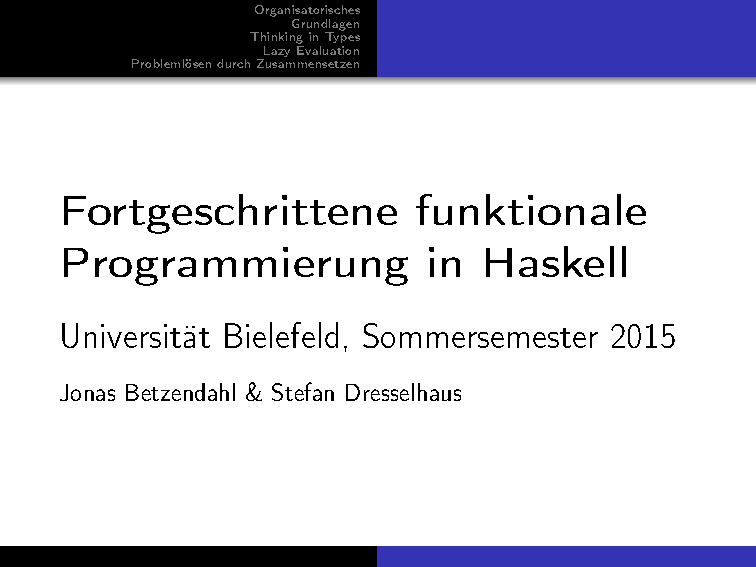
\includepdf[pages=-]{lecture1.pdf}

\subsection*{Vorlesung 2:}
\label{v2}
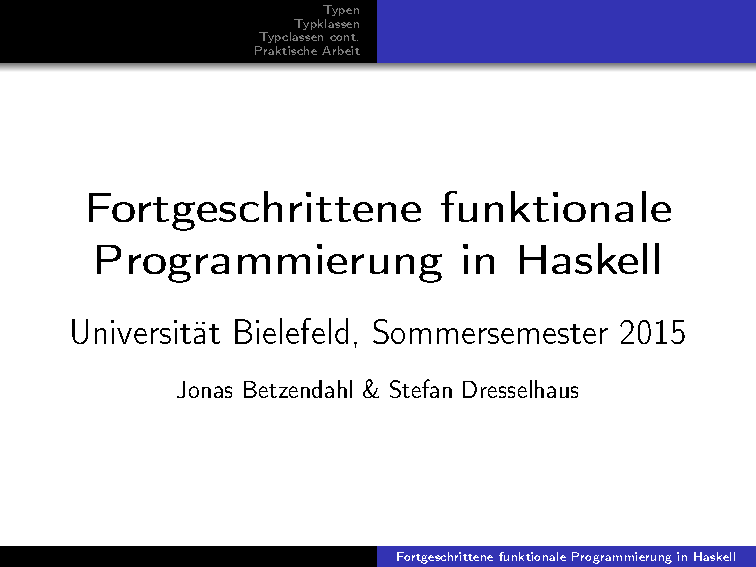
\includepdf[pages=-]{lecture2.pdf}

\subsection*{Vorlesung 3:}
\label{v3}
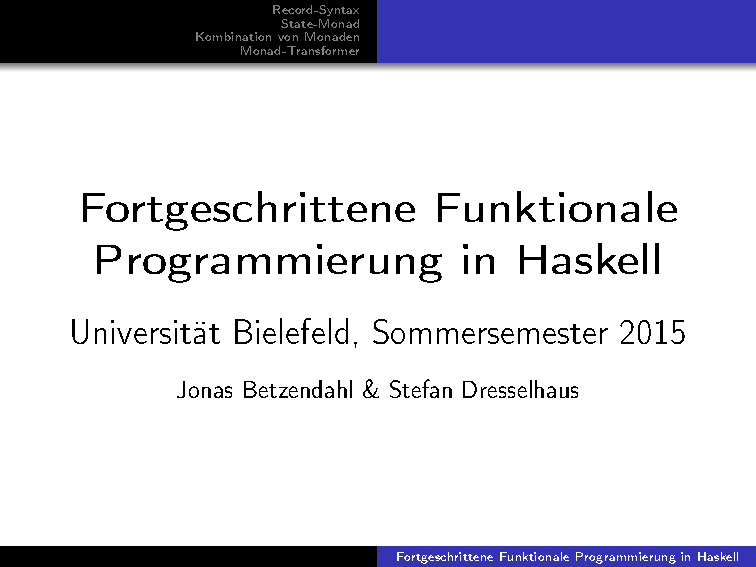
\includepdf[pages=-]{lecture3.pdf}

\subsection*{Vorlesung 4:}
\label{v4}
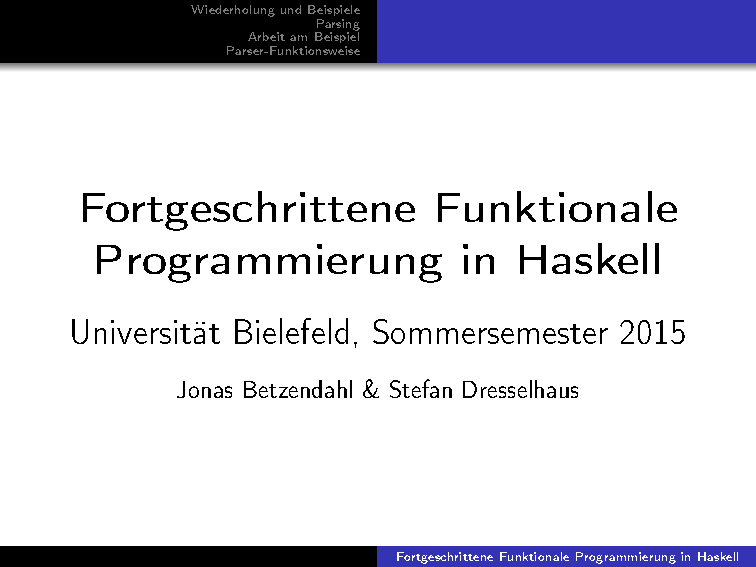
\includepdf[pages=-]{lecture4.pdf}

\subsection*{Vorlesung 5:}
\label{v5}
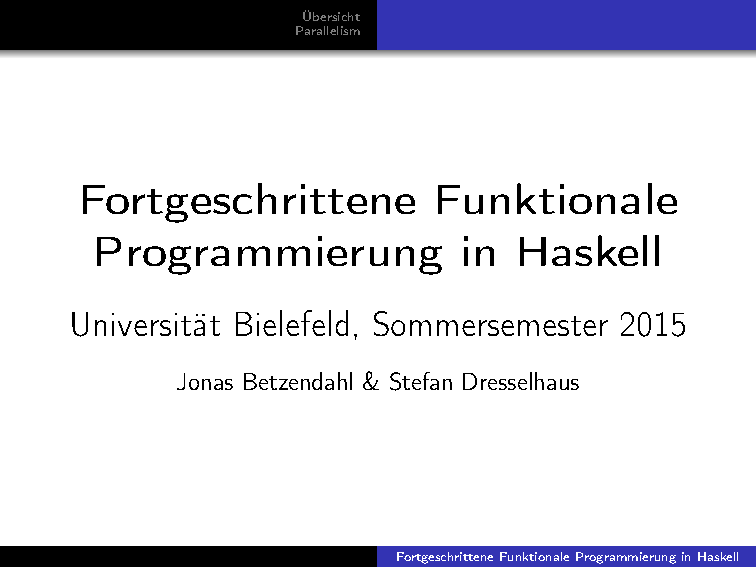
\includepdf[pages=-]{lecture5.pdf}

\subsection*{Vorlesung 6:}
\label{v6}
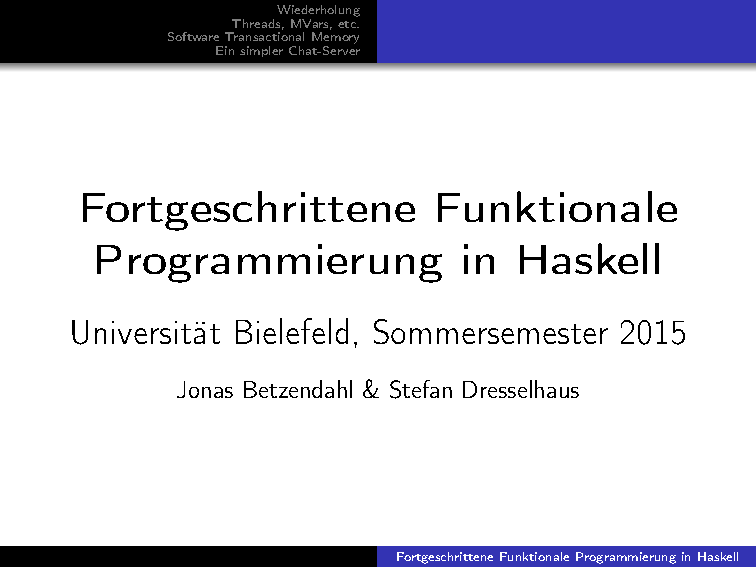
\includepdf[pages=-]{lecture6.pdf}

\subsection*{Vorlesung 7:}
\label{v7}
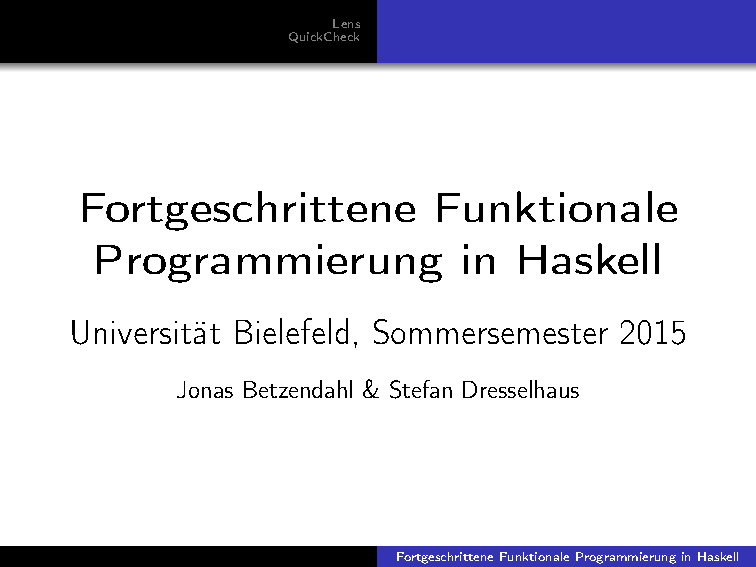
\includepdf[pages=-]{lecture7.pdf}

\subsection*{Vorlesung 8:}
\label{v8}
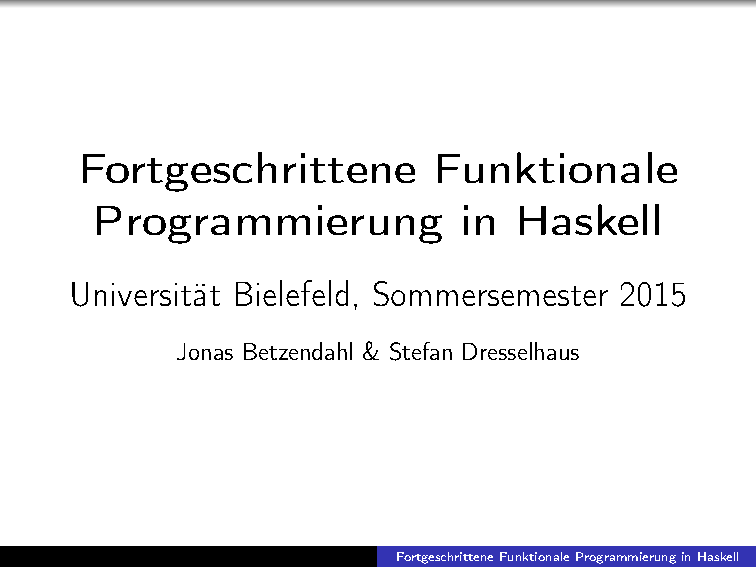
\includepdf[pages=-]{lecture8.pdf}

\subsection*{Vorlesung 9:}
\label{v9}
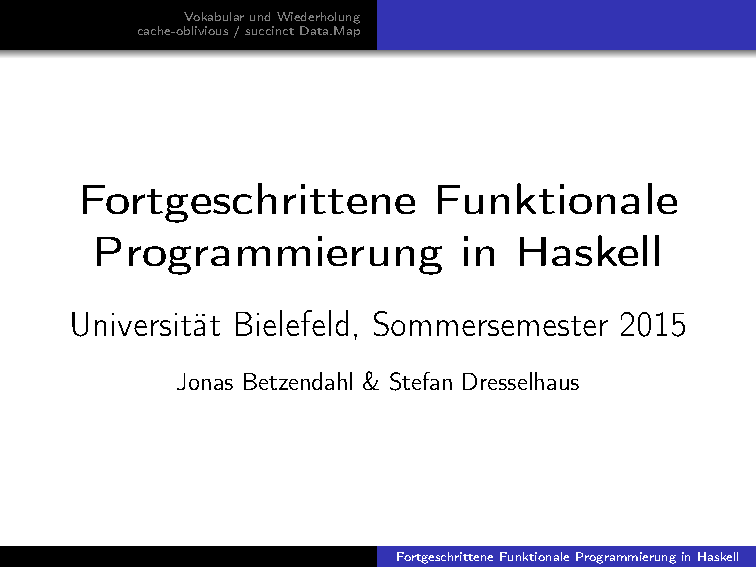
\includepdf[pages=-]{lecture9.pdf}

\subsection*{Vorlesung 10:}
\label{v10}
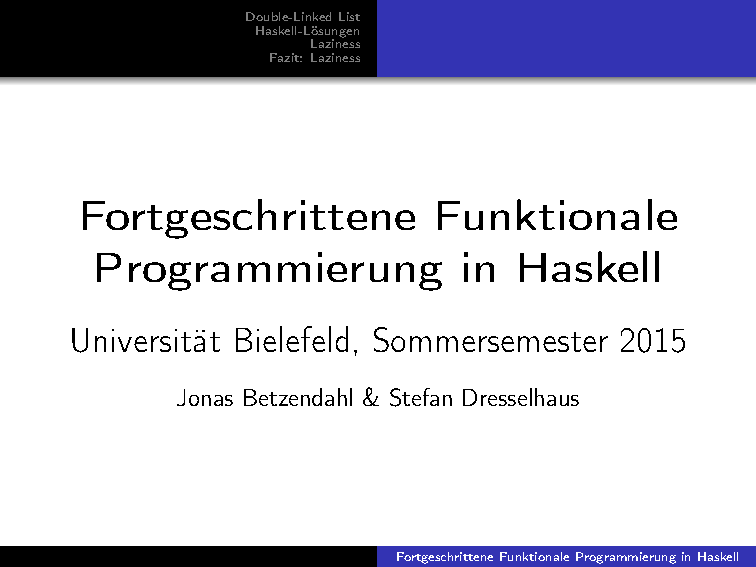
\includepdf[pages=-]{lecture10.pdf}

\subsection*{Vorlesung 11:}
\label{v11}
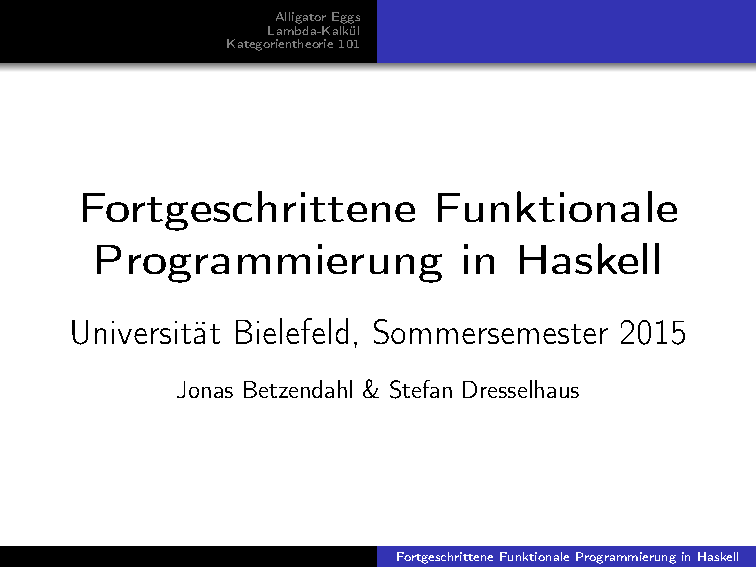
\includepdf[pages=-]{lecture11.pdf}

\end{document}